\subsubsection{Training of a network}\label{training}
As a summary of seen so far, four different elements are necessary to create a network:

\begin{itemize}
\item Input values: Information with which a data or a data set is to be predicted.
\item Structure of the network: This is information that must be known a priori before creating the model. It has different properties:
\begin{itemize}
    \item Number of layers: The higher the number of layers, the longer it will take the model to compute the $y$ output vector because the more calculations it will have to perform. The number of layers together with the number of neurons per layer are important parameters, since a very low number in the model and this will not have a good accuracy. On the contrary a very high number can produce what is known as overfitting (see section \ref{overfitting}).
    
    \item Number of neurons in each layer: It should be noted that the number of neurons in the last layer will be the size of the $y$ vector, i.e. the number of labels that the model will predict.
    \item Activation function for each layer.
    \item Network architecture
\end{itemize}
\item The matrices $W$: These are matrices that collect the information associated with each layer on the weights $w$ and $b$ of each neuron in the network.
\end{itemize}

$W$ matrices are matrices with randomly created values. The network training process will try to optimise these matrices so that the resulting $y$ vector is as accurate as possible. To be able to train a model it is necessary to have previously a dataset with a set of vectors $x$ and their real value. The amount of data we provide to the model to learn is related to the accuracy of the model. With the example described in the table \ref{tab:houses}, we could use the columns: text type, text coordinates, text \textit{lc}, text \textit{m2} and text \textit{r} to predict the value of the price.
\newline


Basically, the network initialises the $W$-matrix randomly. The model given a vector $x$ makes all the calculations for each neuron and returns a vector $y$. $y$ is what the model has predicted. This process is known as forward-pass.
\newline

For the network to learn, it first needs to know if it has made a mistake and the magnitude of the error. If the magnitude of this error is very large, the $W$ values should be adjusted to minimise the error. On the other hand, if the error is small, the $W$ values will not be adjusted much because making an adjustment in $W$ can cause a slight improvement in that prediction, but it can disregard other predictions that the model has made previously and were also quite accurate. The elegance of this algorithm is that it finds a balance between adjusting values so that the network learns and at the same time not misadjusting too much so that the network decompensates in its global learning. It is the application of the imitation of human learning, an error with a great impact will have to modify future behaviours, an error without impact can be ignored or incorporate changes proportionate to the impact.
\newline


The error is quantified with a function called cost function or loss function explained in section \ref{costfunction}. From the value of the error, an algorithm will be used to try to calculate the responsibility of each neuron in this error and thus be able to adjust the weights and biases associated with this neuron. This algorithm is called backpropagation and is explained in section \ref{backpropagation}.
\newline

It can be thought that this process can be repeated infinitely until a perfect model is obtained, but as seen in section \ref{overfitting} this can cause the network to memorise the dataset that is used for training and not have the capacity to generalise. Therefore, it is not only a matter of executing the algorithm, but also of performing certain optimisations and considering several concepts such as: the selection of the activation function, design of the input and output vector, metrics to be used, among others.
\newline

\label{p:company_backpropagation}

As an analogy to understand the backpropragation algorithm, the hierarchy of a company can be used. This company, after a disastrous quarter, produces a summary of the results. These results are equivalent to the error that the model produces. The CEO (the last layer of the network) will try to be accountable to the managers. These managers will in turn deal with other managers with less responsibility and these in turn will deal with managers below them and so on until they reach the last level in the company (spreading the error to the most basic layers). Subsequently, the company will produce a report studying the responsibility of each person in the result of the quarter (which in the backpropagation algorithm is known as the gradient vector). This report will reach the human resources department, which will try to modify the behaviour of each worker in the company according to their responsibility in the error.
\newline

In the following diagram you can visualise the process that takes place to train a neural network:
\begin{figure}[H]
    \centering
    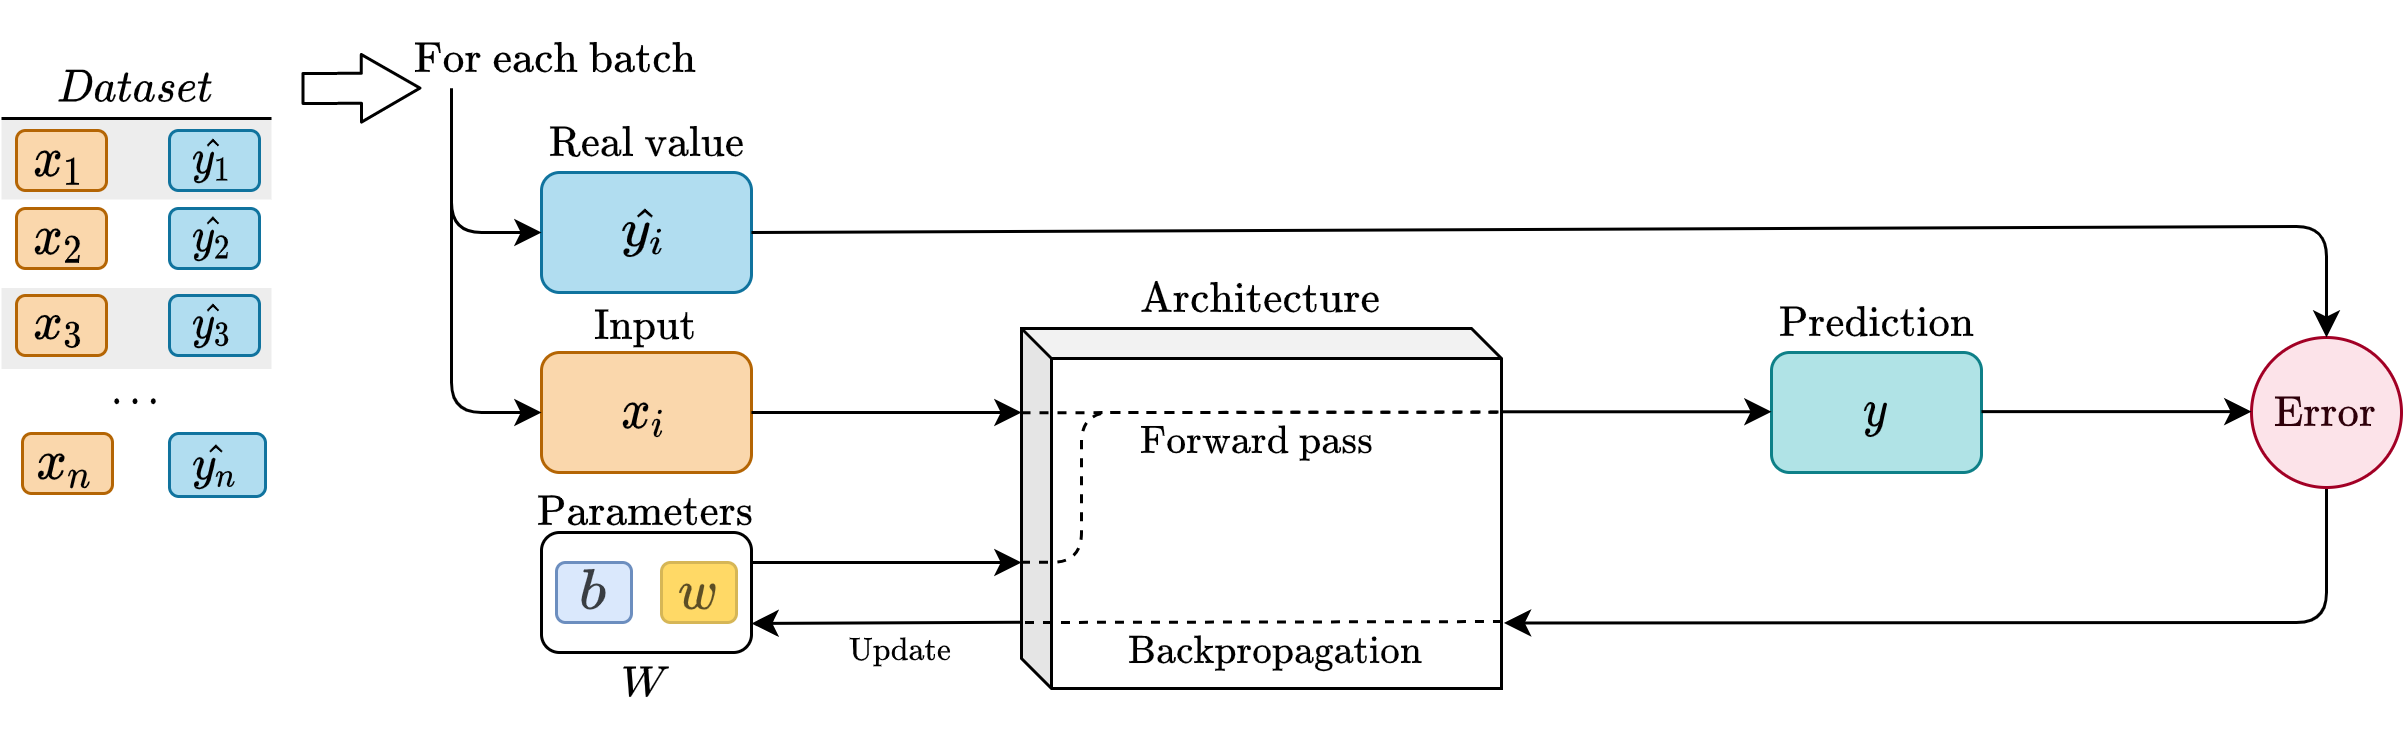
\includegraphics[width=15cm]{images/state-of-art/training/training.png}
    \caption{Training process of a neural network}
    \label{fig:error_regression}
\end{figure}

Training a network is an iterative process. In each iteration, or also known as epoch, a set of data will be taken from the training dataset at random. Each of these datasets taken for each epoch is called a batch and the size of the batch is usually a parameter set by the user.
\newline

The size of a batch is usually 32, 64 or 128 values. In each epoch, the model will only work with these data. It will predict a value for each of the inputs and together with the real value, the cost function, the backpropagation algorithm and the gradient decrease, the W matrices will be adjusted iteratively.